\documentclass{article}
\usepackage[UTF8]{ctex}
\usepackage{mathtools}
\usepackage{amsthm}
\usepackage{amsfonts}
\usepackage{float}
\usepackage{tikz}
\usepackage{graphicx}
\usepackage{indentfirst} % 使首段也缩进
\usepackage{forest}
\setlength{\parindent}{2em} % 设置首行缩进为两个汉字宽度
\everymath{\displaystyle}


\begin{document}
\setcounter{page}{0}
\tableofcontents
\newpage

\section{需求分析}

\subsection{具体需求}
\noindent
需求1:图书管理员需要有个图书管理系统来方便管理与查询图书和用户的信息。需要支持的操作有:添加书籍、添加用户、浏览书籍信息、浏览用户信息、删除书籍信息、删除用户信息、恢复出厂设置等。\\
需求2:需要有设置和修改密码的功能以保证图书管理系统的安全性。\\
% 需求3:需要防止误触误删导致的信息丢失。\\
需求3:需要有个向导来帮助管理员操作系统.\\\\

\subsection{根据需求需要实现的功能}
图书与用户信息增加功能:图书管理员可以添加新用户信息:ID和姓名,可以添加新书籍的信息:书籍ID,书名,作者,ISBN,出版年份。

图书与用户显示浏览功能:展示所有图书信息,展示所有用户信息,此外还包括用户当前借阅书籍数目,具体借阅书籍的信息,书籍的当前借阅者

图书与用户信息删除功能:管理员有权限删除书籍信息和用户信息。

恢复出厂设置功能:管理员可以一键恢复图书管理系统初始状态的信息。

密码设置与修改功能:管理员登录必须输入密码,并且可以修改密码。

UI功能:图书管理系统拥有美观的用户界面,管理员可以移动光标,系统上方有显示当前位于什么功能界面,系统下方还有操作指引,方便管理员清楚如何使用这些功能\\
\subsection{具体功能实现}
\subsubsection{输入功能实现}
输入功能主要通过cin实现,然后通过重载运算符\textgreater{}\textgreater{}用于用户输入数据的写入,接受一个结构实例对象并通过一个属于类的成员函数,并将其添加入类中的存储器中,以此来存储和显示用户的信息。\\
\subsubsection{输出功能实现}
输出则主要通过cout实现,然后通过重载运算符\textless{}\textless{},用于用户输入数据的写入,接受一个结构实例对象并通过一个属于类的成员函数,并将其添加入类中的存储器中,以此来存储和显示用户信息。\\
\subsubsection{核心处理逻辑}
(1)接收输入用户信息,图书信息的User类和Book类的实例对象,将其存储在以ID为键的unordered\_map中,记录存储输入的信息。

(2)遍历这个存储信息的unordered\_map容器,将容器中的数据写入文件,打印出所存信息。

(3)通过ID对图书和用户进行检索。

(4)获取器函数,在Book类与User类中声明定义,返回所存储的图书信息,封装了对图书信息的访问。

(5)各种帮手函数,比如获取书籍或用户信息表格等,为UI的显示提供数据支持。
\subsubsection{UI界面}

(1)UI界面主要是通过UI文件夹中的内容来实现的,table文件中包含了系统的各个功能模块,管理员可以通过光标移动来选择不同的功能模块。界面上方标题栏显示当前所在的功能界面,下方有操作指引,方便管理员清楚如何使用这些功能。

(2)UI文件夹分的文件主要分为两类:component 和 page。前者主要实现各种可在各个页面中复用的组件的功能,如按钮、输入框等,后者主要实现各个页面的布局和功能。通过这些文件的组合,实现了一个美观且易于操作的用户界面。
\subsubsection{数据存储}

使用文件,将数据写入文件中保存,支持永久保存功能,即使在退出系统后数据仍能得以保存,支持静态数据操作。\\
\section{系统设计说明}

\begin{figure}[H]
  \centering
\resizebox{0.5\textwidth}{!}{
  \begin{forest}
  for tree={
      font=\sffamily,
      grow=east,
      draw,
      rounded corners,
      edge={-latex},
      parent anchor=east,
      child anchor=west,
      l sep=15pt,
      s sep=25pt, % 增大节点间纵向距离
      align=left,
      edge path={
        \noexpand\path [draw, \forestoption{edge}] (!u.parent anchor) -- +(5pt,0) |- (.child anchor)\forestoption{edge label};
      },
  }
  [图书管理系统
    [登陆密码, yshift=-250pt
      [输入密码, yshift=-250pt]
      [修改密码, yshift=-250pt]
      [输入密码, yshift=-250pt]
      [修改密码, yshift=-250pt]
    ]
    [退出系统]
    [增加信息
      [图书
        [ID]
        [书名]
        [作者]
        [ISBN]
        [出版年份]
      ]
      [用户
        [ID]
        [姓名]
      ]
    ]
    [浏览信息
      [图书
        [当前借阅者]
      ]
      [用户
        [借阅数]
      ]
    ]
    [删除信息]
    [UI
      [光标移动]
      [操作功能指引]
    ]
    [恢复出厂设置]
  ]
  \end{forest}
}
\caption{图书管理系统思维导图}
\end{figure}
\section{系统操作}
\subsection{登录系统}

我们设计了一个简单的登录系统,管理员需要输入密码才能进入系统。密码可以通过修改功能进行更改,以保证系统的安全性。登录成功后,管理员可以进行各种操作,如添加图书、添加用户、浏览信息等。
这是为了防止未授权用户访问系统,确保只有管理员可以进行管理操作。以下是系统的登录界面。

\begin{figure}[H]
    \centering
    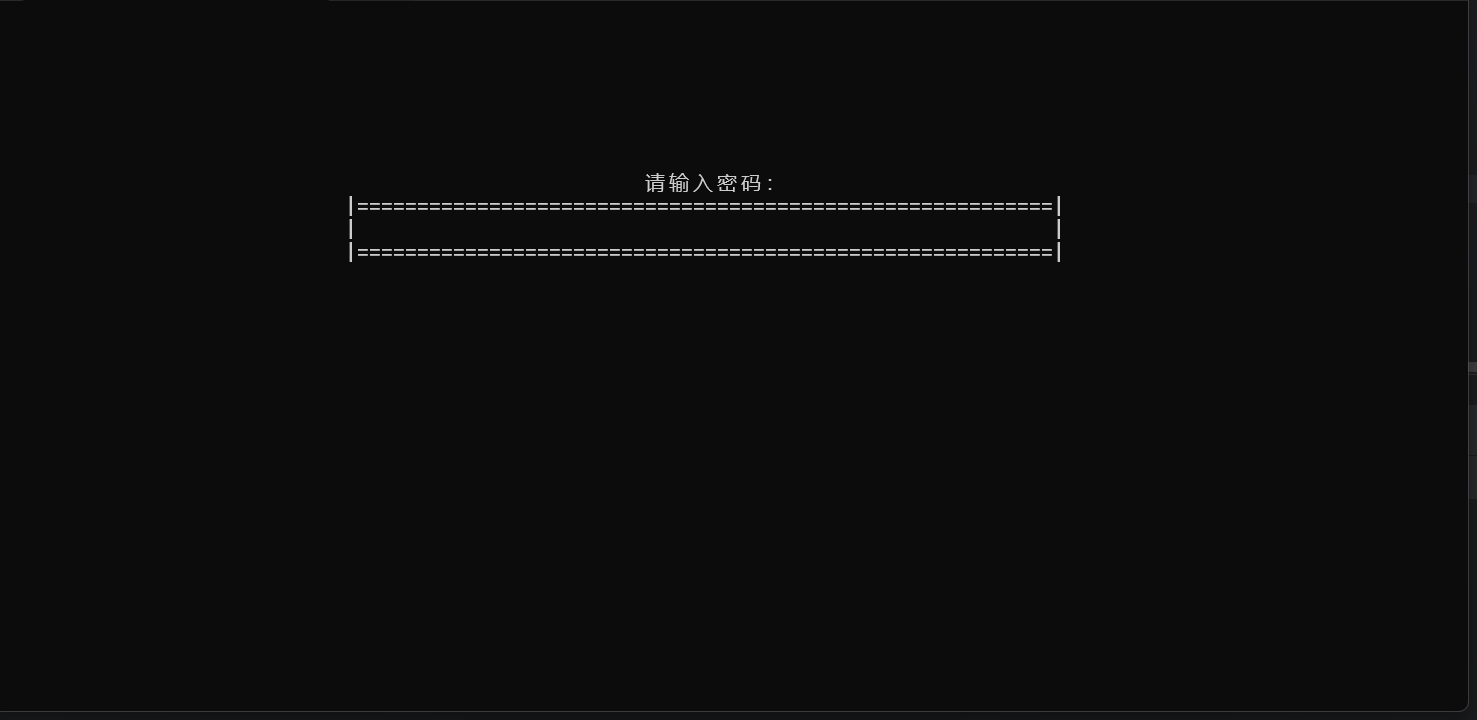
\includegraphics[width=0.8\textwidth]{loading.png}
    \caption{系统登录界面示意图}
\end{figure}

\subsection{操作界面演示}

这是一个简单的UI界面,管理员可以通过光标移动来选择不同的功能模块。界面上方标题栏显示当前所在的功能界面,下方有操作指引,方便管理员清楚如何使用这些功能。具体是按Enter键来选择确认功能,按Esc键返回上一级菜单。
负责上下移动的光标则是使用\textgreater{}符号表示

\begin{figure}[H]
    \centering
    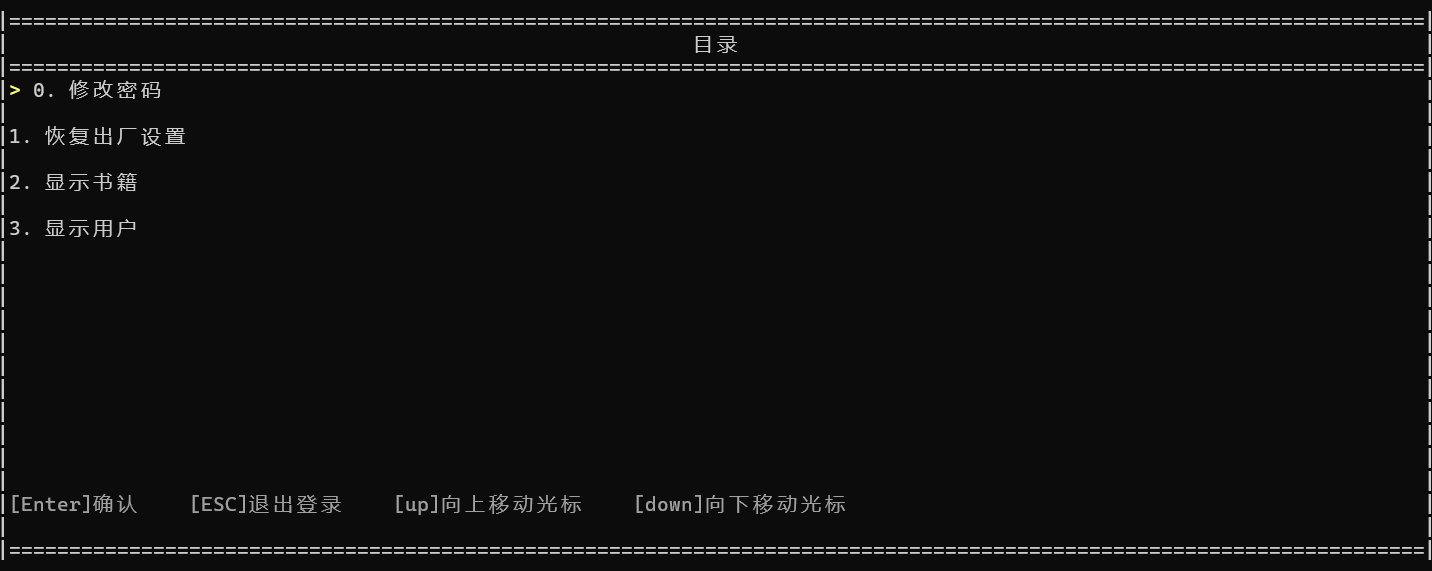
\includegraphics[width=0.8\textwidth]{system.png}
    \caption{系统操作界面示意图}
\end{figure}

\subsection{用户信息查寻与图书信息查寻}
管理员可以通过系统浏览所有用户信息和图书信息。用户信息包括用户ID和姓名,图书信息包括图书ID、书名、作者、ISBN和出版年份等。管理员可以查看当前借阅者和借阅数目等信息。只需把光标移动到显示用户和
显示书籍,点击Enter键即可进入详情界面。

\begin{figure}[H]
    \centering
    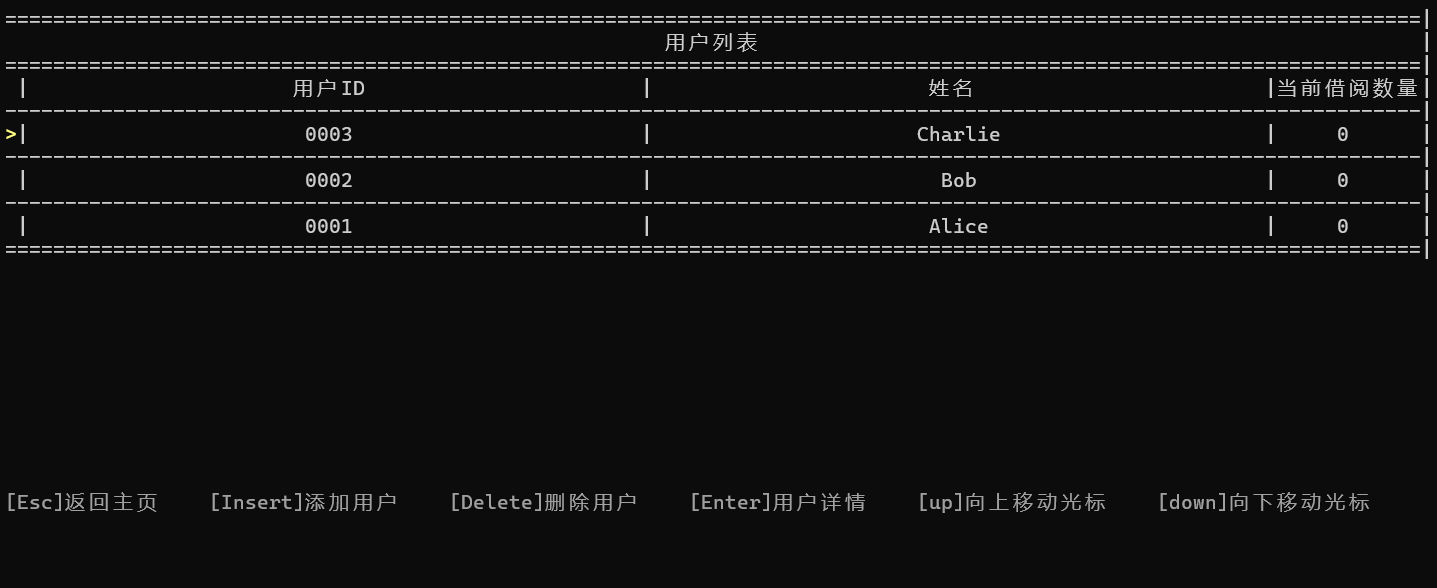
\includegraphics[width=0.8\textwidth]{user.png}
    \caption{用户界面示意图}
\end{figure}

\begin{figure}[H]
    \centering
    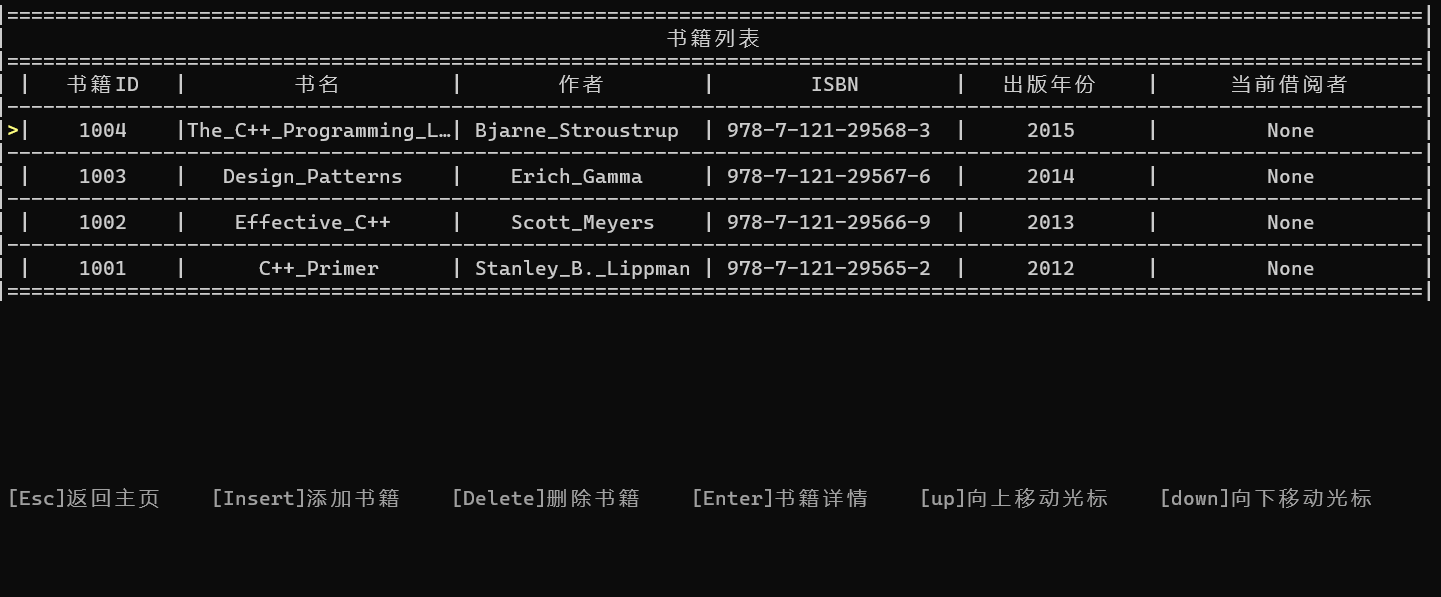
\includegraphics[width=0.8\textwidth]{book.png}
    \caption{书籍界面示意图}
\end{figure}


按照下方的操作指引,管理员可以按Insert键添加书籍和用户按Delete键删除书籍和用户,按Esc键返回上一级菜单。
\subsection{借阅书籍的的操作}

在用户界面选择借书者,按Enter进入二级页面,按Insert键进入借阅界面,点击Enter即可借阅选定的图书,按Delete键还书。

\begin{figure}[H]
    \centering
    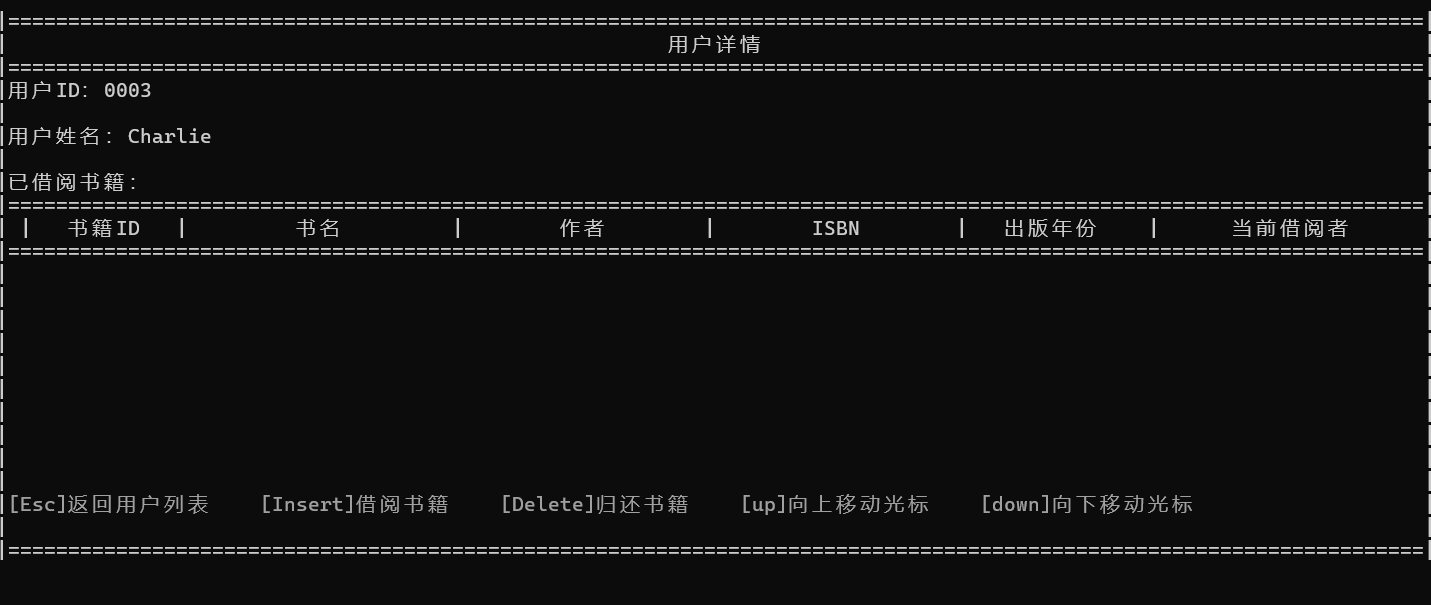
\includegraphics[width=0.8\textwidth]{borrow.png}
    \caption{借阅界面示意图}
\end{figure}

\begin{figure}[H]
    \centering
    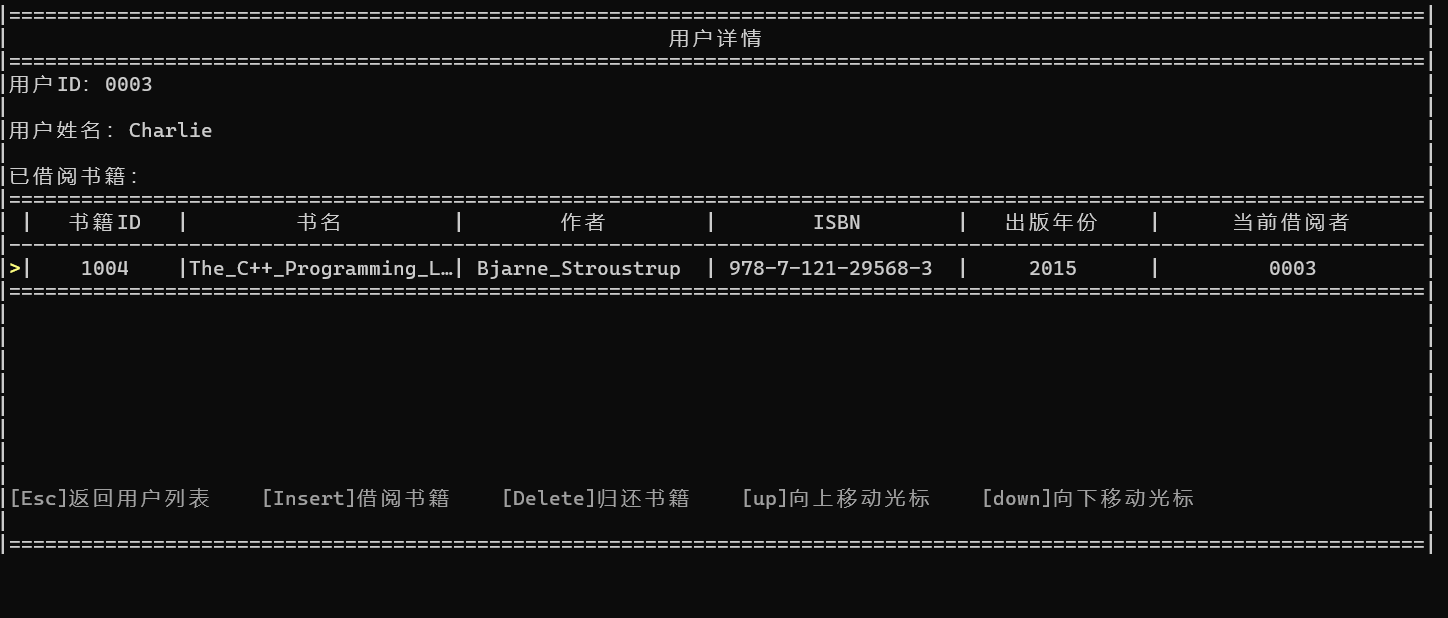
\includegraphics[width=0.8\textwidth]{manipulate.png}
    \caption{归还界面示意图}
\end{figure}

\subsection{用户和图书的信息}
点开用户和图书的二级页面即可显示用户和图书的所有信息,包括用户ID、姓名,图书ID、书名、作者、ISBN和出版年份等信息。管理员可以通过光标移动来选择不同的用户或图书,按Enter键查看详细信息。
\subsection{恢复出厂设置}
管理员可以通过恢复出厂设置功能将系统重置到初始状态。此功能会清除所有用户和图书信息,并将系统恢复到最初的设置。管理员只需在主界面选择恢复出厂设置,按Enter键确认即可。
\subsection{退出系统}
管理员可以通过退出系统功能来安全地退出图书管理系统。只需在主界面选择退出系统,按Enter键确认即可。退出后,所有未保存的数据将被写入文件,确保系统的安全性。

\section{总结}

本次关于图书馆管理系统的程序设计,是我们小组基于图书馆管理的实际需求,设计并实现了一个简单的图书管理系统。该系统包括了图书信息和用户信息的添加、浏览、删除等功能,
并且提供了密码设置与修改功能以保证系统的安全性。通过思维导图的方式,我们清晰地展示了系统的结构和各个功能模块之间的关系。在设计过程中,我们注重了用户体验,确保系统界面美观且易于操作。
管理员可以通过简单的操作来管理图书和用户信息,帮助管理员更好地使用系统。该系统中利用C++中对类的定义,设计了Library类来实现图书管理系统的核心功能。
Library类包含了图书和用户信息的管理方法,并且通过文件操作实现了数据的持久化存储。其中我们设计了User类和Book类来分别表示用户和图书信息。User类包含了用户的ID和姓名等基本信息,
而Book类则包含了图书的ID、书名、作者、ISBN和出版年份等信息。通过这些类,我们能够方便地对用户和图书进行管理。此外还设计了辅助函数、辅助类来实现系统的功能。
为了对用户和图书的数据进行安全封装,我们使用文件对系统信息进行储存以实现永久保存功能,即使是在退出系统后数据仍能得以保存。此外,考虑到学习成本,我们对系统界面进行了美观处理,
设计了简洁明了的UI界面,我们把UI界面写在table文件中,模块化处理,避免了代码冗余。通过该系统,我们可以对用户及图书的信息进行登记,增改,删除。可以浏览数据库中所有的用户与图书信息,
查看当前借阅者和借阅数目等。管理员可以通过输入密码来登录系统,并且可以修改密码以保证系统的安全性。系统还提供了恢复出厂设置的功能,以便在需要时重置系统到初始状态。
尽管在整个过程中出现了不少困难和错误,我们最终还是圆满地完成了此次的课程程序设计,并且取得了一定的进步。

综上所述,本次关于图书馆管理系统的程序设计,是我们小组基于图书馆管理的实际需求,设计并实现了一个简单的图书管理系统。该系统包括了图书信息和用户信息的添加、浏览、删除等功能,
并且提供了密码设置与修改功能以保证系统的安全性。通过思维导图的方式,我们清晰地展示了系统的结构和各个功能模块之间的关系。

\newpage
\section{附录}

\end{document}
